\subsection{B.2. 不同脚手架下的思考强度}\label{b.2.-reasoning-efforts-across-scaffolds}

在图 11 的全部六个面板中，提高思考强度设置都会拉长轨迹：在每个脚手架--基准
组合中，每条轨迹的平均输出 token 数都随努力水平单调增长。Pass@1 只是松散地
跟随这一增长。它总体上有所提升，但响应并非单调，在大多数面板的中间档位出现
平台期和回落。三种脚手架的校准方式也不同：在 DeepSWE v1.1 上，Claude Code
的曲线最平缓、额外消耗的 token 相对较少，而 DeepSeek Harness（Minimal）起点
最低并在最大的 token 开销下收益最多，mini-SWE 介于两者之间。在 Terminal-Bench
v2.1 上，三种脚手架被压缩进一条很窄的带内，最大努力水平下的排序偏向 DeepSeek
Harness（Minimal），其后依次是 mini-SWE 和 Claude Code：当任务接近饱和时，
脚手架选择的重要性至少与强度档位相当。

\subsection{B.3. 各思考强度档位下推理基准的详细结果}\label{b.3.-detailed-results-of-reasoning-benchmarks-across-reasoning-efforts}

图 12 显示，思考强度设置能在全部八个基准上一致地提供对输出长度与准确率的平滑、
可控调节；这些基准覆盖竞赛数学、科学问答、开放领域知识与代码。在长度一侧，
把努力水平从 25 提高到 100 会在每个基准上可预期地缩放平均响应 -- 统一的
2.0--3.1$\times$ 增长，在 AIME 2026 上每条响应从 4.6k 到 11.4k token，在
MathArena Apex 2025 上从 29.1k 到 86.1k -- 没有失控增长或异常，因此任何档位的
计算成本都可以事先估算。准确率沿同样的平滑轨迹变化，并在每个基准上都朝正确
方向响应，没有任何基准随努力增加而退化：MathArena Apex 2025 提升 +40.3
分（25.3\%$\to$65.6\%），Apex 2025 Shortlist 提升 +11.5，而即便是已经饱和的基准
也保持稳定（GPQA Diamond +1.3，LiveCodeBench +2.6），AIME 2026 达到完整的
100\%。因此该模型暴露了一个单一、可靠的旋钮，以受控且可预期的方式移动
成本--准确率工作点，使每个部署都能选择与其延迟和计算预算匹配的强度档位，
而不牺牲准确率。\footnote{mini-swe-agent, commit 04d809ceab9d}


\subsection{C. 思考强度控制中的指数 token 惩罚}\label{c.-exponential-token-penalty-in-reasoning-effort-control}

标量努力变量为成本--质量权衡提供了部署时的控制手段，而不施加硬性的 token
预算。在强化学习期间，较低的强度档位施加更强的 token 惩罚，而较高的强度档位
允许更多的计算。本节对指数惩罚调度给出简化的动机说明。

对于一条在强度档位 \(b ,\) 下生成 \(\ell\) 个推理 token 的轨迹，其长度
扣减为

\[
r ^ { \mathrm { l e n } } ( \ell , b ) = - \operatorname* { m i n } \left\{ C _ { \mathrm { m a x } } , k ( b ) \frac { \ell } { L _ { \mathrm { n o r m } } } \right\} ,\tag{11}
\]

其中 \(L _ { \mathrm { n o r m } }\) 是参考长度，\(C _ { \mathrm { m a x } }\)
对扣减设上限。与强度档位相关的 token 惩罚系数为

\[
k ( b ) = k _ { 0 } \exp \left( - \frac { b - b _ { \mathrm { m i n } } } { \tau } \right) ,\tag{12}
\]

其中 \(k _ { 0 }\) 是最低强度档位 \(b _ { \mathrm { min } }\) 下的惩罚系数，
\(\tau\) 控制惩罚衰减的速率。

为了说明这一选择的动机，考虑一个固定问题 $x$。设 \(p _ { x } ( \ell )\)
表示其在生成 $\ell$ 个推理 token 后被解出的概率。在未达上限的区域，
定义首选推理长度 $\ell_x^*(b)$ 为

\[
\ell _ { x } ^ { * } ( b ) \in \arg \operatorname* { m a x } _ { \ell \geqslant 0 } \left[ p _ { x } ( \ell ) - k ( b ) \frac { \ell } { L _ { \mathrm { n o r m } } } \right] .\tag{13}
\]

对于内部最优解，一阶条件为

\[
p _ { x } ^ { \prime } \big ( \ell _ { x } ^ { * } ( b ) \big ) = \frac { k ( b ) } { L _ { \mathrm { n o r m } } } ,\tag{14}
\]

其中
\(p _ { x } ^ { \prime } ( \ell ) = d p _ { x } ( \ell ) / d \ell\) 是
额外推理带来的解出概率的边际提升。

我们假设这一边际收益在相关运行区间内近似按指数衰减：

\[
p _ { x } ^ { \prime } ( \ell ) \approx a _ { x } \exp \left( - \frac { \ell } { s _ { x } } \right) ,\tag{15}
\]

其中 \(a _ { x } > 0\) 是随实例变化的尺度，\(s _ { x } > 0\) 决定衰减速率。
将式 (12) 和 (15) 代入式 (14) 得

\[
\ell _ { x } ^ { \ast } ( b ) \approx C _ { x } - s _ { x } \log k _ { 0 } + \frac { s _ { x } } { \tau } ( b - b _ { \mathrm { m i n } } ) ,\tag{16}
\]

其中
\(C _ { x } = s _ { x } \log ( a _ { x } L _ { \mathrm { n o r m } } )\)
与 $b$ 无关。因此，在此局部模型下，指数惩罚调度会在所要求努力水平与首选
推理长度之间产生简单的一阶仿射趋势。

对于两个强度档位 \(b _ { 2 } > b _ { 1 }\) ，对应的预测长度差为

\[
\ell _ { x } ^ { \ast } ( b _ { 2 } ) - \ell _ { x } ^ { \ast } ( b _ { 1 } ) \approx \frac { s _ { x } } { \tau } ( b _ { 2 } - b _ { 1 } ) .\tag{17}
\]

因此，\(k _ { 0 }\) 主要控制朝更短推理方向的整体压力，而 $\tau$ 控制对努力
水平的预测敏感度。

此推导是一种局部的奖励层面近似，并非声称实测平均长度必然是线性或逐点单调的。
实际行为可能偏离，因为努力指令可以直接改变推理策略，生成是随机的，智能体
轨迹包含不同轮数的交互，且子组奖励归一化会改变优化强度。该分析还假设解在
内部、惩罚上限不生效。一旦达到上限，边际 token 惩罚变为零，超限区域必须
单独考虑。

\begin{figure}[htbp]
\centering
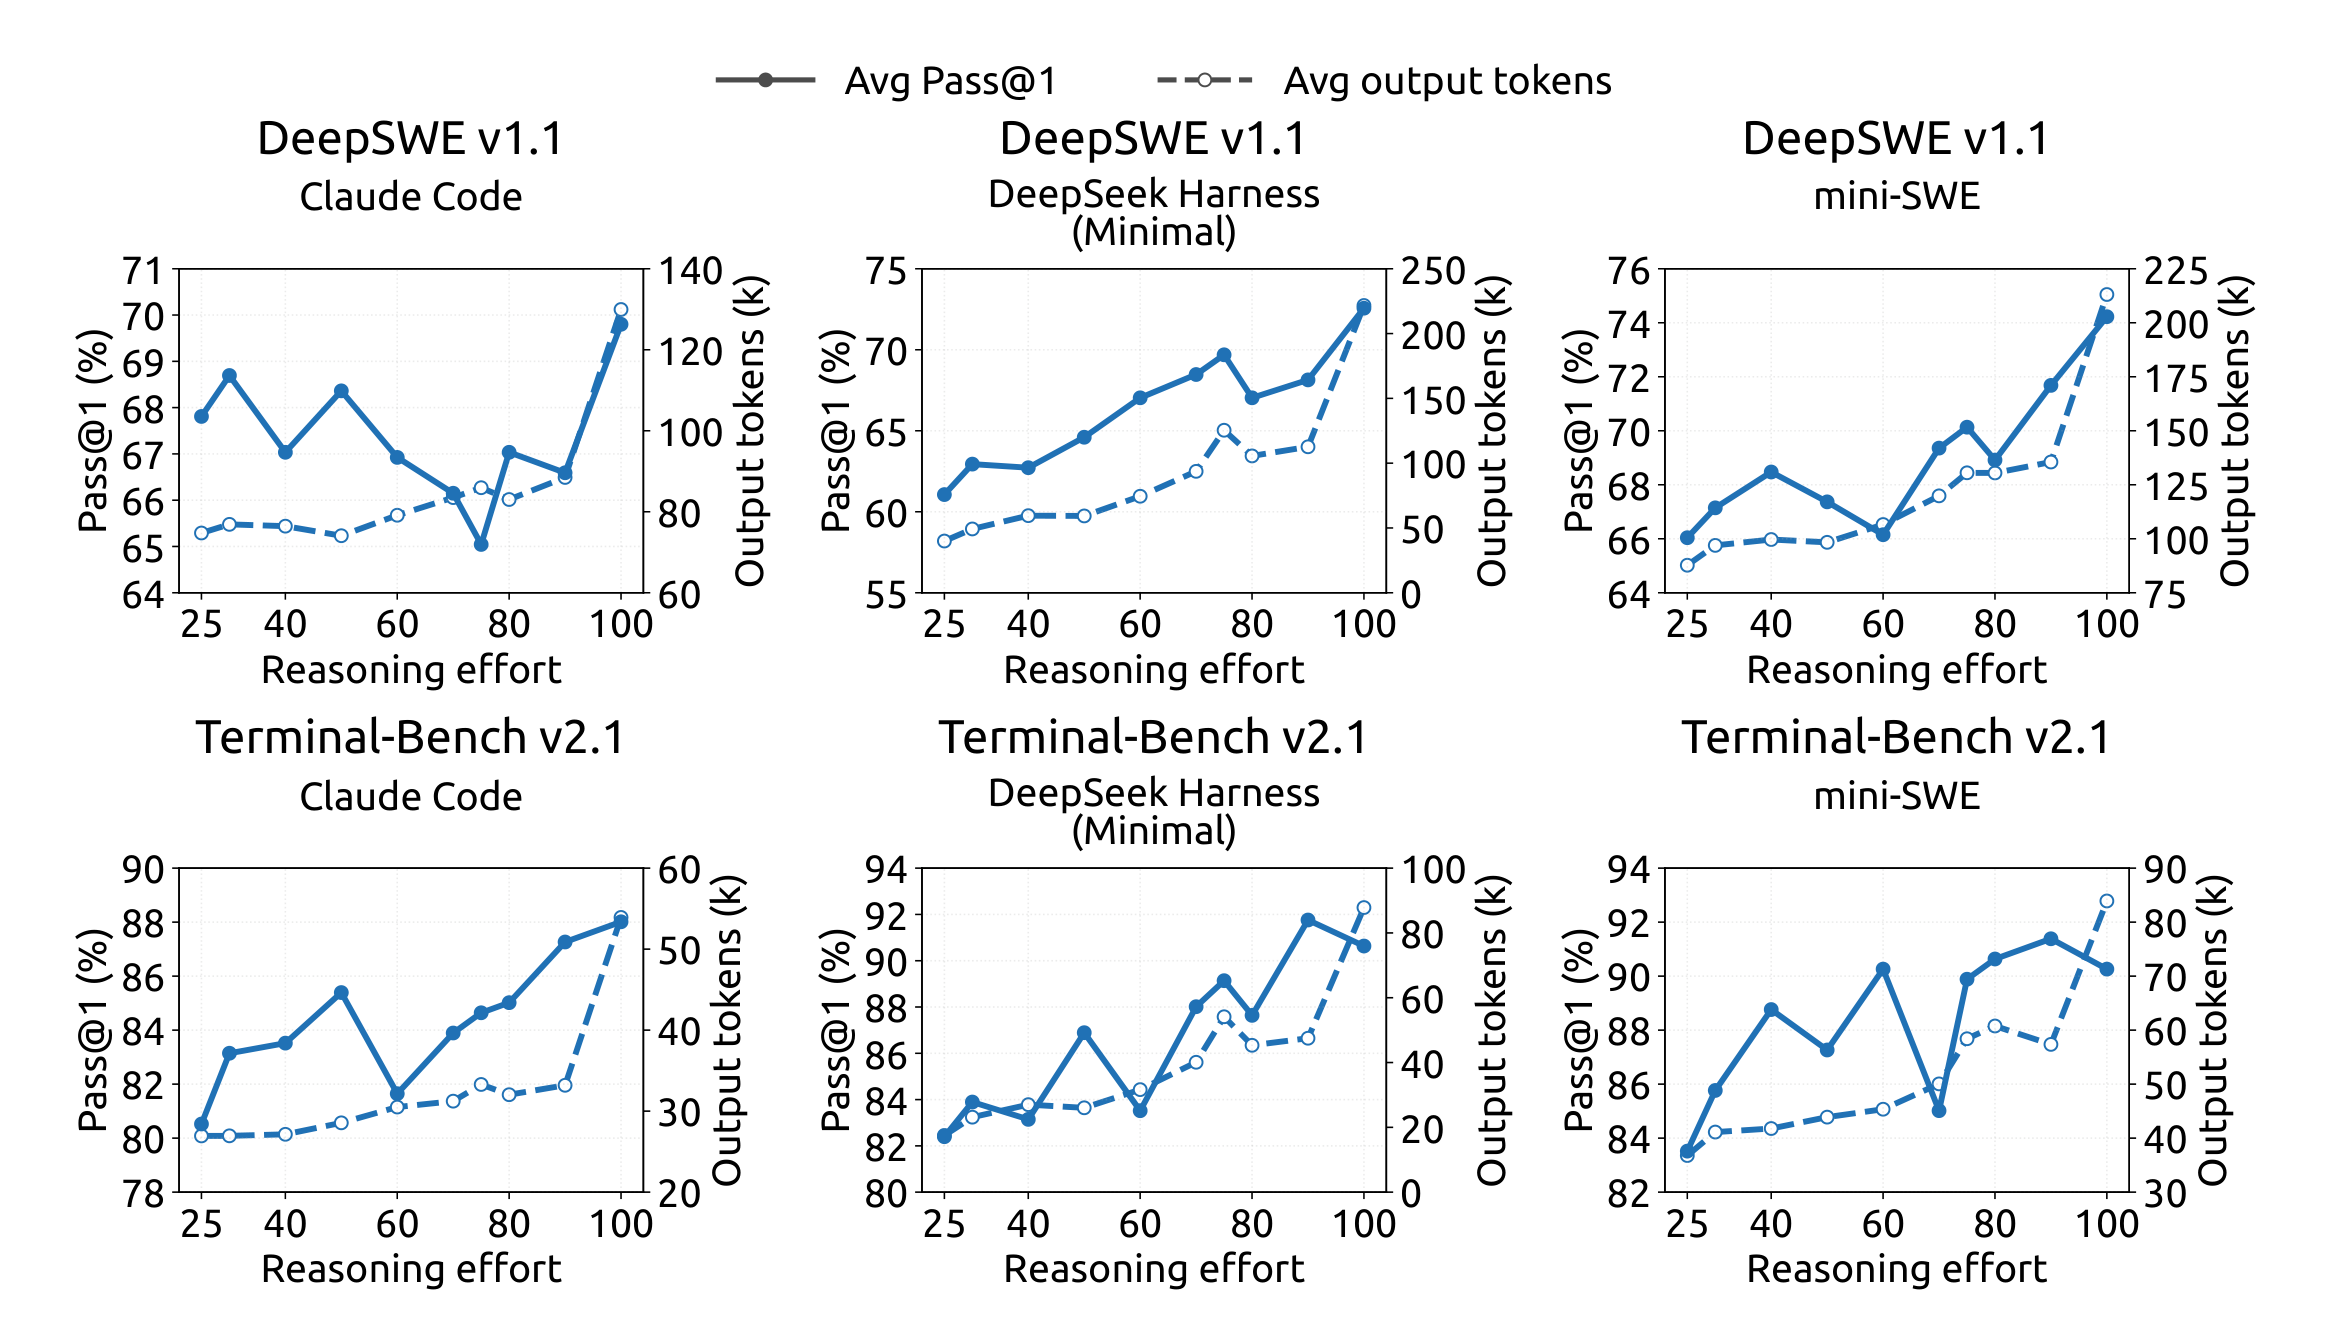
\includegraphics[width=\linewidth]{images_hi/fig11}
\caption{思考强度会一以贯之地拉长轨迹长度，但与各编码脚手架上的准确率仅呈弱相关。每个面板将 Pass@1（\%，实线，左轴）和每条轨迹的平均输出 token 数（k，虚线，右轴）与思考强度设置对应绘图，涵盖 DeepSWE v1.1（上排）和 Terminal-Bench v2.1（下排）在三种智能体脚手架（Claude Code、DeepSeek Harness（Minimal）与 mini-SWE）下的结果。所有面板均来自同一 checkpoint。}
\label{fig:11}
\end{figure}
\begin{figure}[htbp]
\centering
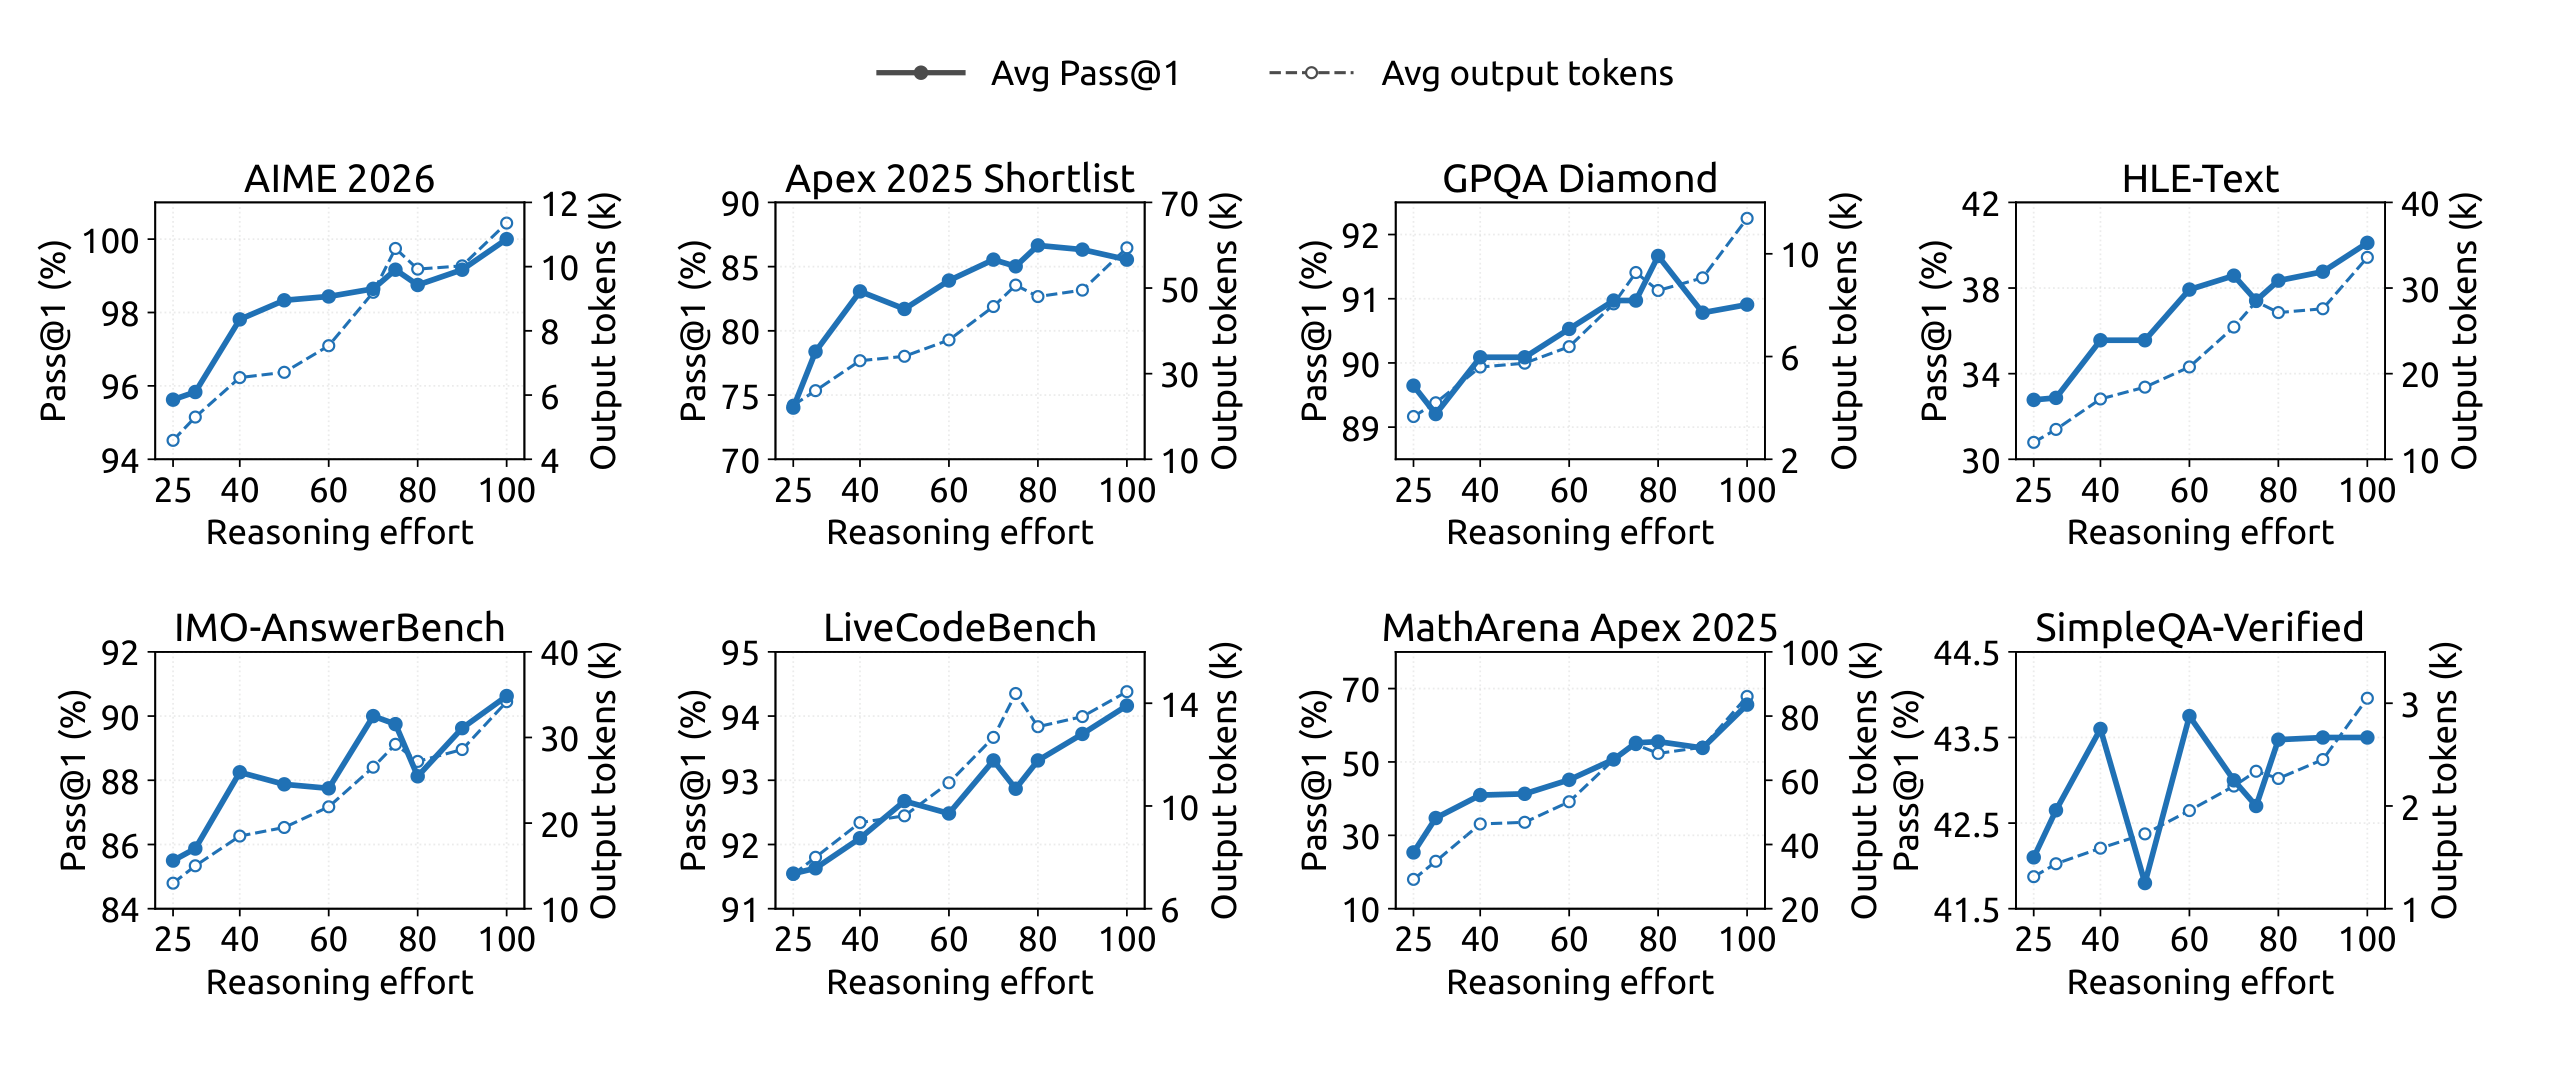
\includegraphics[width=\linewidth]{images_hi/fig12}
\caption{八个推理密集型基准上性能与输出长度随思考强度的变化。每个面板在思考强度取值从 25 变化到 100 时，绘制 Pass@1（实线，左轴）和每条响应的平均输出 token 数（虚线，右轴）。}
\label{fig:12}
\end{figure}